\chapter{Manual de Usuario para el Docente}
\label{chap:mandocente}

Los docentes serán los que tendrán la responsabilidad de crear y mantener los diferentes chats que puedan existir en la aplicación móvil. Por tanto, es relevante que se conozca el funcionamiento de la misma, a fin de llevar a cabo dicha tarea de una manera adecuada.

\subsection*{Iniciar Sesión}
Lo primero que muestra la aplicación la primera vez que se utiliza en un \textit{smartphone} es la pantalla de bienvenida, donde se inicia el procedimiento de identificación e inicio de sesión del usuario (Figura \ref{fig:inicioappdocente}). En esta pantalla se muestran tres botones, siendo los dos primeros dedicados a los usuarios de las familias, mientras que el último (<<Soy Docente>>), está dedicado específicamente al inicio de sesión por parte de los docentes registrados. Al pulsar, se mostrará un diálogo preguntando si se desea acceder mediante correo electrónico y contraseña o usando el número de teléfono asociado al docente (Figura \ref{fig:preguntadocente}).

\begin{figure}[!h]
	\centering
	\begin{minipage}{.5\textwidth}
		\centering
		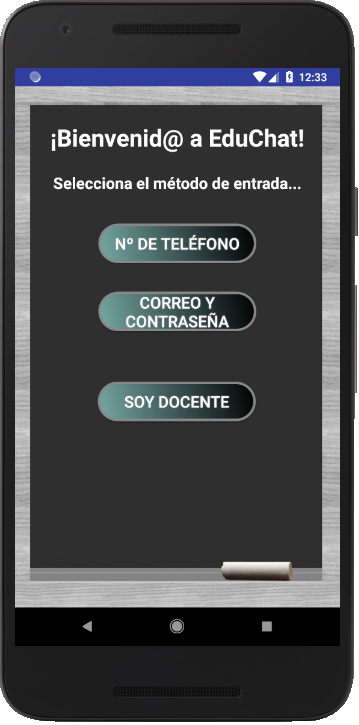
\includegraphics[width=0.6\textwidth]{/manuales/docente/inicioapp}
		\caption{Pantalla de Inicio de EduChat}
		\label{fig:inicioappdocente}
	\end{minipage}%
	\begin{minipage}{.5\textwidth}
		\centering
		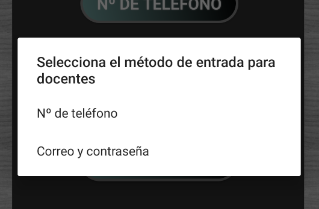
\includegraphics[width=0.8\textwidth]{manuales/docente/preguntadocente}
		\caption{Pregunta de Inicio de Sesión}
		\label{fig:preguntadocente}
	\end{minipage}
\end{figure}

\clearpage

En el caso en el que se elija iniciar sesión mediante el número de teléfono, se mostrará una actividad en la que se deberá introducir el número de teléfono y pulsar el botón <<Enviar Código>> (Figura \ref{fig:iniciotfnodocente}). Unos instantes después se recibirá un \acs{SMS} con un código que se deberá introducir en la aplicación para poder finalizar el inicio de sesión. Por el contrario, si se desea iniciar sesión haciendo uso del correo electrónico y una contraseña, el docente deberá introducir ambos valores en la pantalla que se muestra (Figura \ref{fig:iniciocorreodocente}). Si es la primera vez que se inicia sesión, la contraseña que se introduzca será la que quede registrada en la base de datos. No obstante, existe la posibilidad de cambiarla en caso de que así se desee o se haya olvidado mediante la opción <<¿Has olvidado tu contraseña?>>, en cuyo caso se deberá introducir el correo electrónico y pulsar el botón de <<Enviar Correo>> para recibir un mensaje en la dirección escrita. Dicho mensaje contendrá un enlace con instrucciones a seguir para cambiar la contraseña de acceso.

\begin{figure}[!h]
	\centering
	\begin{minipage}{.5\textwidth}
		\centering
		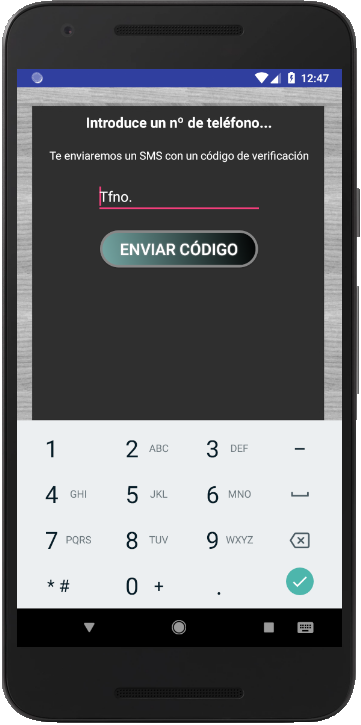
\includegraphics[width=0.6\textwidth]{/manuales/docente/iniciotfno}
		\caption{Pantalla de Inicio con Número \\ de Tfno.}
		\label{fig:iniciotfnodocente}
	\end{minipage}%
	\begin{minipage}{.5\textwidth}
		\centering
		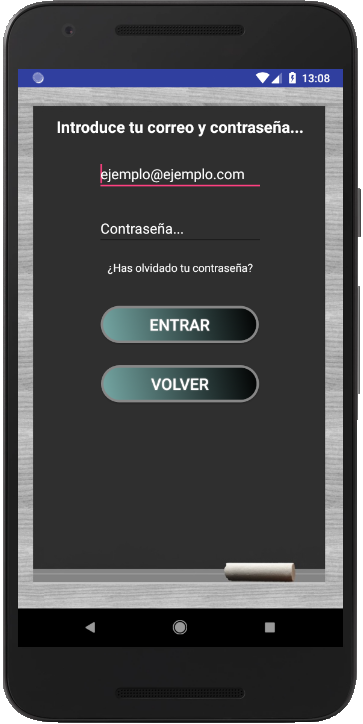
\includegraphics[width=0.6\textwidth]{manuales/docente/iniciocorreo}
		\caption{Pantalla de Inicio con Correo y Contraseña}
		\label{fig:iniciocorreodocente}
	\end{minipage}
\end{figure}

\clearpage

\subsection*{Crear y Eliminar Chats}
Una vez que se ha iniciado sesión y se ha accedido a la aplicación, el docente podrá crear nuevos chats mediante el menú situado en la esquina superior derecha, representado con tres puntos alineados verticalmente, seleccionando la opción <<Crear nuevo chat...>>. A continuación, deberá escoger un nombre para el nuevo chat, así como los integrantes que conformarán el mismo (Figura \ref{fig:crearchat}). Una vez hecho esto, se finalizará la creación pulsando el botón <<Crear Chat>>. Este nuevo chat se mostrará en la pantalla principal de la aplicación, así como cualquier otro del que se sea miembro. Además, los docentes podrán eliminar los chats que hayan creado, realizando una pulsación larga sobre su nombre en la lista de la pantalla principal, tras lo que se mostrará un diálogo confirmando la eliminación. (Figura \ref{fig:eliminarchat}).

\begin{figure}[!h]
	\centering
	\begin{minipage}{.5\textwidth}
		\centering
		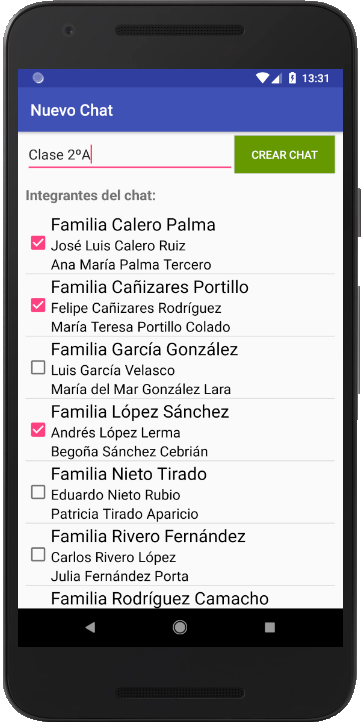
\includegraphics[width=0.6\textwidth]{/manuales/docente/crearchat}
		\caption{Pantalla de Creación de Chat}
		\label{fig:crearchat}
	\end{minipage}%
	\begin{minipage}{.5\textwidth}
		\centering
		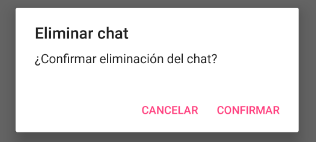
\includegraphics[width=0.8\textwidth]{manuales/docente/eliminar}
		\caption{Confirmación de Borrado de Chat}
		\label{fig:eliminarchat}
	\end{minipage}
\end{figure}

\clearpage

\subsection*{Ver Perfil y Cambiar Imagen}
Mediante el menú principal de la aplicación también se permite visualizar la información del usuario, así como la imagen de perfil, si tuviera una definida (Figura \ref{fig:perfildocente}). Si se desea establecer una nueva imagen, se podrá hacer mediante el botón <<Cambiar Imagen de Perfil>>, pudiendo escoger alguna fotografía de la galería. Por el contrario, si se desea eliminar la imagen de perfil, se podrá realizar pulsando el botón <<Eliminar Imagen de Perfil>>, restableciendo el avatar por defecto.

\begin{figure}[!h]
	\begin{center}
		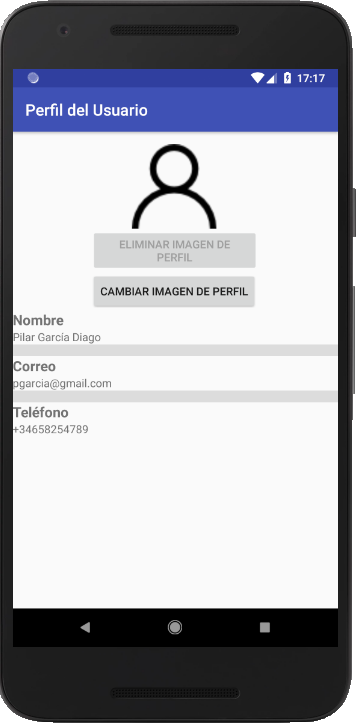
\includegraphics[width=0.4\textwidth]{/manuales/docente/perfil}
		\caption{Pantalla de Perfil}
		\label{fig:perfildocente}
	\end{center}
\end{figure}

\clearpage

\subsection*{Ver Información del Chat}
Todos los chats poseen un apartado en el que se muestra su información. Se puede acceder pulsando el botón <<Info.>>, que se encuentra en la esquina superior derecha de cada uno. Desde esta pantalla se puede visualizar el nombre del grupo y renombrarlo mediante el botón dedicado a ello, así como disponer de una lista con los integrantes de este (Figura \ref{fig:infochatdocente}). Asimismo, se puede visualizar al lado de cada integrante un número en forma de porcentaje, que representa el tono que ha tenido este en el chat, siendo 0\% el peor resultado y el 100\% el mejor. De igual manera, se podrá visualizar el tono individual de cada mensaje con colores rojo, naranja, amarillo y verde, en orden creciente de puntuación. Además se podrá acceder a la información de cada familia pulsando sobre el nombre de estas (Figura \ref{fig:infointegrantedocente}).

\begin{figure}[!h]
	\centering
	\begin{minipage}{.5\textwidth}
		\centering
		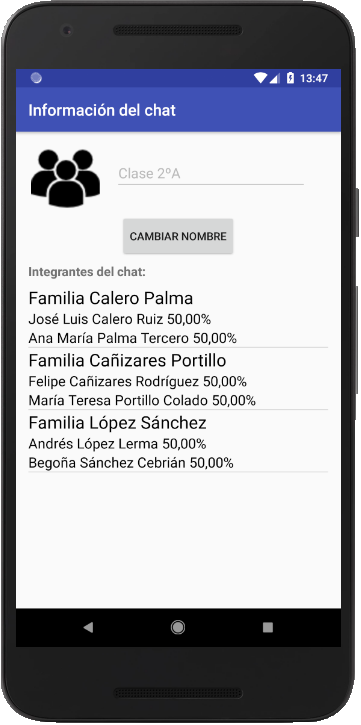
\includegraphics[width=0.6\textwidth]{/manuales/docente/infochat}
		\caption{Pantalla de Información \\ del Chat}
		\label{fig:infochatdocente}
	\end{minipage}%
	\begin{minipage}{.5\textwidth}
		\centering
		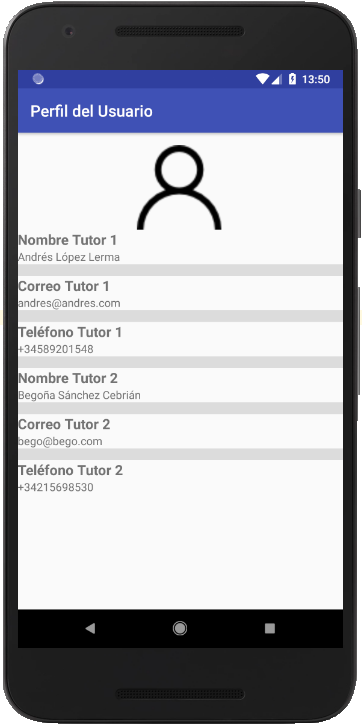
\includegraphics[width=0.6\textwidth]{manuales/docente/infointegrante}
		\caption{Pantalla de Información de \\ Integrante}
		\label{fig:infointegrantedocente}
	\end{minipage}
\end{figure}

\clearpage

\subsection*{Crear Eventos de Calendario}
Un docente puede crear un evento de calendario para avisar a los integrantes del chat de acontecimientos futuros, tales como reuniones, charlas, excursiones, etc. Para ello, bastará pulsar sobre el botón (+) que se encuentra en la esquina inferior izquierda (Figura \ref{fig:creareventodocente}), lanzando la aplicación de calendario con todos los correos electrónicos de los integrantes del chat. Únicamente se debe especificar el nombre del evento, duración o lugar para completar la información de este y que sea de mayor utilidad para los invitados al mismo.

\begin{figure}[!h]
	\begin{center}
		
\includegraphics[width=0.3\textwidth]{/manuales/docente/crearevento}
		\caption{Botón para Crear Evento}
		\label{fig:creareventodocente}
	\end{center}
\end{figure}



